\chapter{Технологический раздел}
\label{cha:impl}

В данном разделе будут описаны средства реализации программного обеспечения, требования к нему, представлены реализации алгоритмов и рассмотрен интерфейс программы.

\section{Требования к программному обеспечению}

Программа должна предоставлять доступ к функционалу:

\begin{itemize}
	\item возможность выбора материала покрытия пола и стен из предложенных вариантов (дерево, бумага(обои), керамика(плитка));
	\item изменение скорости движения частиц;
	\item изменение количества частиц инфекции;
	\item включение и выключение работы модели распространения частиц;
	\item вращение, перемещение и масштабирование модели.
\end{itemize}

\section{Средства реализации}

В качестве языка программирования для реализации курсовой работы использовался язык программирования C++ \cite{cplusplus}, так как он содержит возможности для создания программ с графическим интерфейсом. В качестве среды разработки использовался Qt Creator \cite{qtcreator}.

\section{Реализация алгоритмов}

В листинге \ref{code:brown} представлена реализация алгоритма моделирования броуновского движения.

\begin{lstlisting}[label=code:brown,caption=Реализация вычисления изменения координат центров частиц (броуновское движение)]
void BrownianMotion::setVirusCountAndResetAllIfNeeded(int newVirusCount)
{
	if (virusCount == newVirusCount)
	{
		return;
	}
	virusCount = newVirusCount;
	float sigma = 0.2;
	data = std::vector<std::vector<Vector3f>>(virusCount, std::vector<Vector3f>(SIZE + 1));
	for (int k = 0; k < virusCount; k++)
	{
		data.at(k).at(0) = Vector3f(0.0, 0.0, 0.0);
		data.at(k).at(SIZE) = Vector3f(sigma * getNormalRandom(), sigma * getNormalRandom(), sigma * getNormalRandom());
		for (int j = 1; j <= POWER; j++)
		{
			for (int i = 1; i <= pow(2, (j - 1)); i++)
			{
				int ind = (2 * i - 1) * pow(2, POWER - j);
				int old1 = (i - 1) * pow(2, POWER - j + 1);
				int old2 = i * pow(2, POWER - j + 1);
				data.at(k).at(ind).x = (data.at(k).at(old1).x + data.at(k).at(old2).x) / 2 + sigma * getNormalRandom() / pow(2, (j + 1) / 2);
				data.at(k).at(ind).y = (data.at(k).at(old1).y + data.at(k).at(old2).y) / 2 + sigma * getNormalRandom() / pow(2, (j + 1) / 2);
				data.at(k).at(ind).z = (data.at(k).at(old1).z + data.at(k).at(old2).z) / 2 + sigma * getNormalRandom() / pow(2, (j + 1) / 2);
			}
		}
	}
}
\end{lstlisting}

В листинге \ref{code:processLight} представлена реализация вычисления интенсивности вершины от источников света на сцене.

\begin{lstlisting}[label=code:processLight,caption=Реализация вычисления интенсивности вершины]
float Drawer::processLight(const Vector3f& vert, const Vector3f& norm)
{
	float wholeIntensity = 0;
	float intensity;
	
	size_t lights = scene.getLightSourceCount();
	
	for (size_t i = 0; i < lights; i++)
	{
		intensity = 0;
		LightSourcePoint lsp = scene.getLightSource(i);
		
		Vector3f lightDir = vert - lsp.getPosition();
		
		intensity += lightDir * norm / pow(lightDir.norm(), 2.0);
		intensity *= lsp.getIntensity() * LIGHT_REFLECT;
		
		intensity = fmax(0.0, intensity);
		intensity = fmin(1.0, intensity);
		
		intensity = BG_LIGHT + intensity * (1 - BG_LIGHT);
		
		wholeIntensity += intensity;
	}
	
	if (wholeIntensity == 0)
	wholeIntensity = BG_LIGHT;
	else
	wholeIntensity /= lights;
	
	return wholeIntensity;
}
\end{lstlisting}

В листинге \ref{code:processPoligon} представлен алгоритм вычисления глубины каждой точки полигона и её интенсивности.

\begin{lstlisting}[label=code:processPoligon,caption=Реализация вычисления интенсивности вершины]
void Drawer::processPoligon(Vector3i& t0, Vector3i& t1, Vector3i& t2,
const QColor& color, float& i0, float& i1, float& i2,
float modelAlpha)
{
	if (t0.y == t1.y && t0.y == t2.y)
	return;
	
	if (t0.y > t1.y)
	{
		std::swap(t0, t1);
		std::swap(i0, i1);
	}
	if (t0.y > t2.y)
	{
		std::swap(t0, t2);
		std::swap(i0, i2);
	}
	if (t1.y > t2.y)
	{
		std::swap(t1, t2);
		std::swap(i1, i2);
	}
	
	int total_height = t2.y - t0.y;
	
	for (int i = 0; i < total_height; i++)
	{
		bool second_half = i > t1.y - t0.y || t1.y == t0.y;
		int segment_height = second_half ? t2.y - t1.y : t1.y - t0.y;
		
		float alpha = (float)i / total_height;
		float betta = (float)(i - (second_half ? t1.y - t0.y : 0)) / segment_height;
		
		Vector3i A = t0 + Vector3f(t2 - t0) * alpha;
		Vector3i B = second_half ? t1 + Vector3f(t2 - t1) * betta : t0 + Vector3f(t1 - t0) * betta;
		
		float iA = i0 + (i2 - i0) * alpha;
		float iB = second_half ? i1 + (i2 - i1) * betta : i0 + (i1 - i0) * betta;
		
		if (A.x > B.x)
		{
			std::swap(A, B);
			std::swap(iA, iB);
		}
		
		A.x = std::max(A.x, 0);
		B.x = std::min(B.x, w);
		
		for (int j = A.x; j <= B.x; j++)
		{
			float phi = B.x == A.x ? 1. : (float)(j - A.x) / (float)(B.x - A.x);
			
			Vector3i P = Vector3f(A) + Vector3f(B - A) * phi;
			float iP = iA + (iB - iA) * phi;
			if (P.x >= w || P.y >= h || P.x < 0 || P.y < 0) continue;
			
			if (zBuffer.getDepth(P.x, P.y) < P.z)
			{
				zBuffer.setDepth(P.x, P.y, P.z);
				QColor newColor = QColor(iColor(color.rgba(), iP));
				if (fabs(modelAlpha - 1.0) > EPS)
				{
					newColor = calculateNewColor(newColor, colorCache[P.x][P.y], modelAlpha);
				}
				colorCache[P.x][P.y] = newColor;
			}
		}
	}
}
\end{lstlisting}

\section{Интерфейс работы программного обеспечения}

На рисунке \ref{fig:simple} изображена сцена без частиц вируса.

\begin{figure}[ph!]
	\center{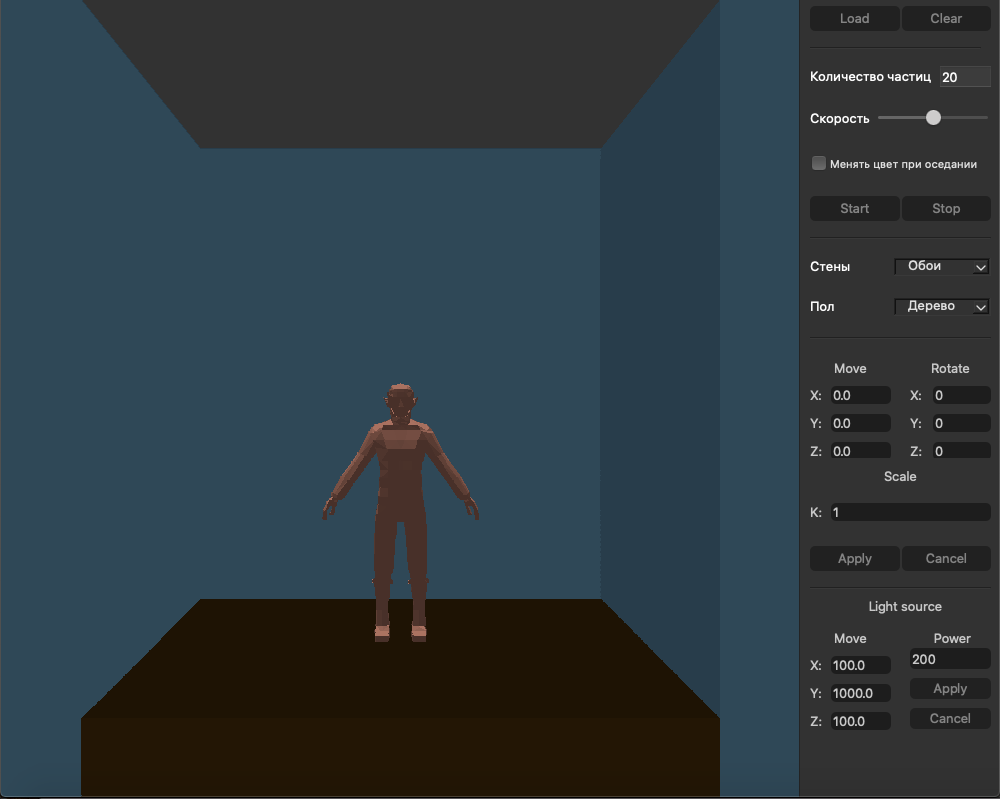
\includegraphics[scale=0.35]{img/scene.png}}
	\caption{Отображение сцены без частиц вируса}
	\label{fig:simple}
\end{figure}

На рисунке \ref{fig:virus_move1} изображено движение частиц.

\begin{figure}[ph!]
	\center{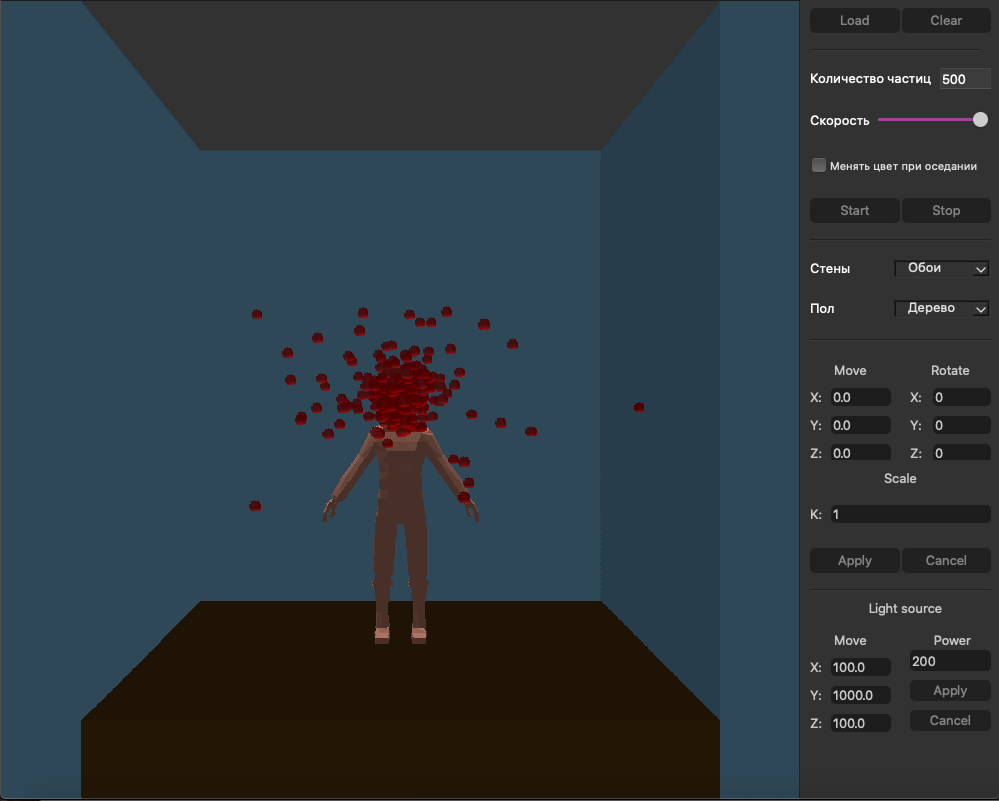
\includegraphics[scale=0.35]{img/movement.png}}
	\caption{Пример движения частиц}
	\label{fig:virus_move1}
\end{figure}

На рисунке \ref{fig:virus_settled} видно, как частицы осели на теле человека и стене и начали тускнеть.

\begin{figure}[ph!]
	\center{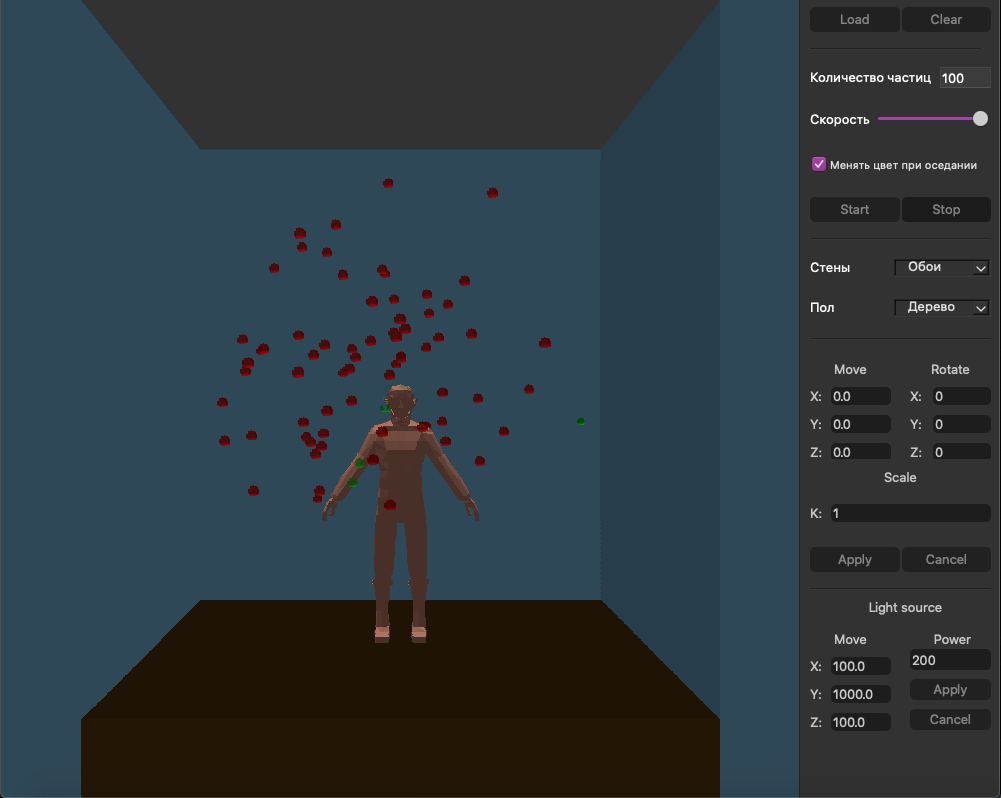
\includegraphics[scale=0.35]{img/settle.png}}
	\caption{Пример оседания и тускнения частиц}
	\label{fig:virus_settled}
\end{figure}

\section*{Вывод}
В данном разделе были перечислены требования к программному обеспечению, средства разработки, с помощью которых была реализована программа, приведены реализации алгоритмов вычисления необходимых параметров для отрисовки сцены, а также алгоритма моделирования броуновского движения.


